% !Mode:: "TeX:UTF-8"

\chapter{相关研究}
第一章简单介绍了复杂网络社团检测的研究现状,包括静态网络社团检测、动态网络社团检测以及动态网络社团演化的研究现状,并简单说明了以上研究的区别以及关联。同时第一章还介绍了城市风险计算的研究现状,以及社团检测在城市风险计算中的重要作用。本章则从具体的方法论角度介绍动态网络社团检测以及社团演化的研究现状与趋势,包括增量聚类、进化聚类和基于模型的聚类方法。为了验证动态社团检测方法的有效性,本章进一步介绍了相关的社团检测评价指标,包含归一化互信息、均方误差和模块度的定义。接着,本章进一步详细介绍城市风险计算的相关研究以及动态社团检测在风险计算中的作用。
\section{动态网络社团检测}

动态网络社团检测本质上包含了静态复杂网络的社团检测(第一个网络快照上)、动态网络社团检测和社团演化分析三个子问题。对于第一个问题可以借用静态网络社团检测的方法完成,而第二个问题则是目前研究者关注的重点,同时第三个问题--社团演化分析则有助于理解社团的演化模式和动态复杂网络的变化规律。如图\ref{fig.3}所示,图中左右两张图是论文引用数据(DBLP数据)在相邻两个时间快照上的社团可视化图,左侧为前一个时间快照,右侧为后一个时间快照,而不同的颜色代表论文所属的研究领域不同,可以看到,下一时刻的社团结构与上一时刻的社团结构变化很大,只有同时融合社团演化规律与动态社团检测方法才能有效的针对动态复杂网络数据进行高精度的社团检测。
\begin{figure}[!htbp]
	\setlength{\abovecaptionskip}{0pt} 
	\setlength{\belowcaptionskip}{10pt} 
	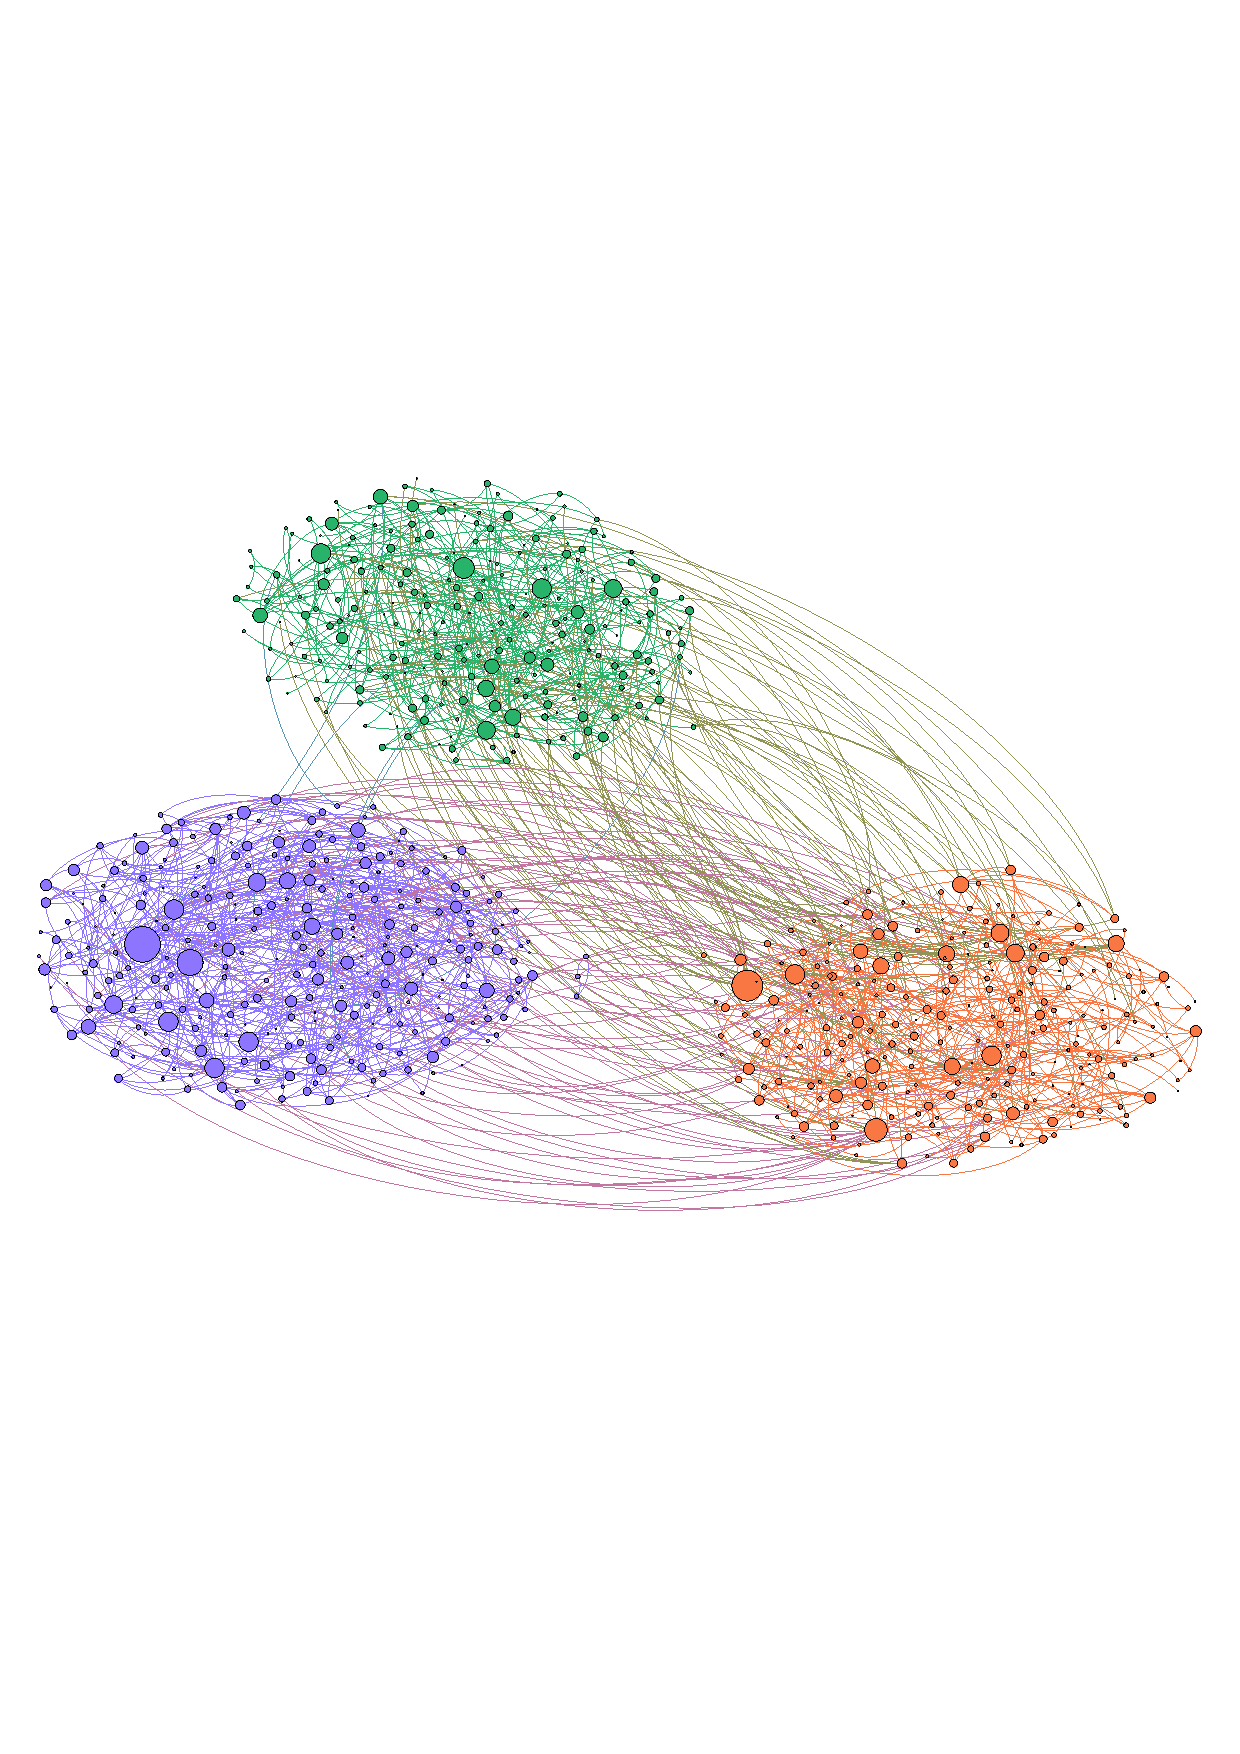
\includegraphics[width=.48\textwidth]{./figure/community1.pdf}
	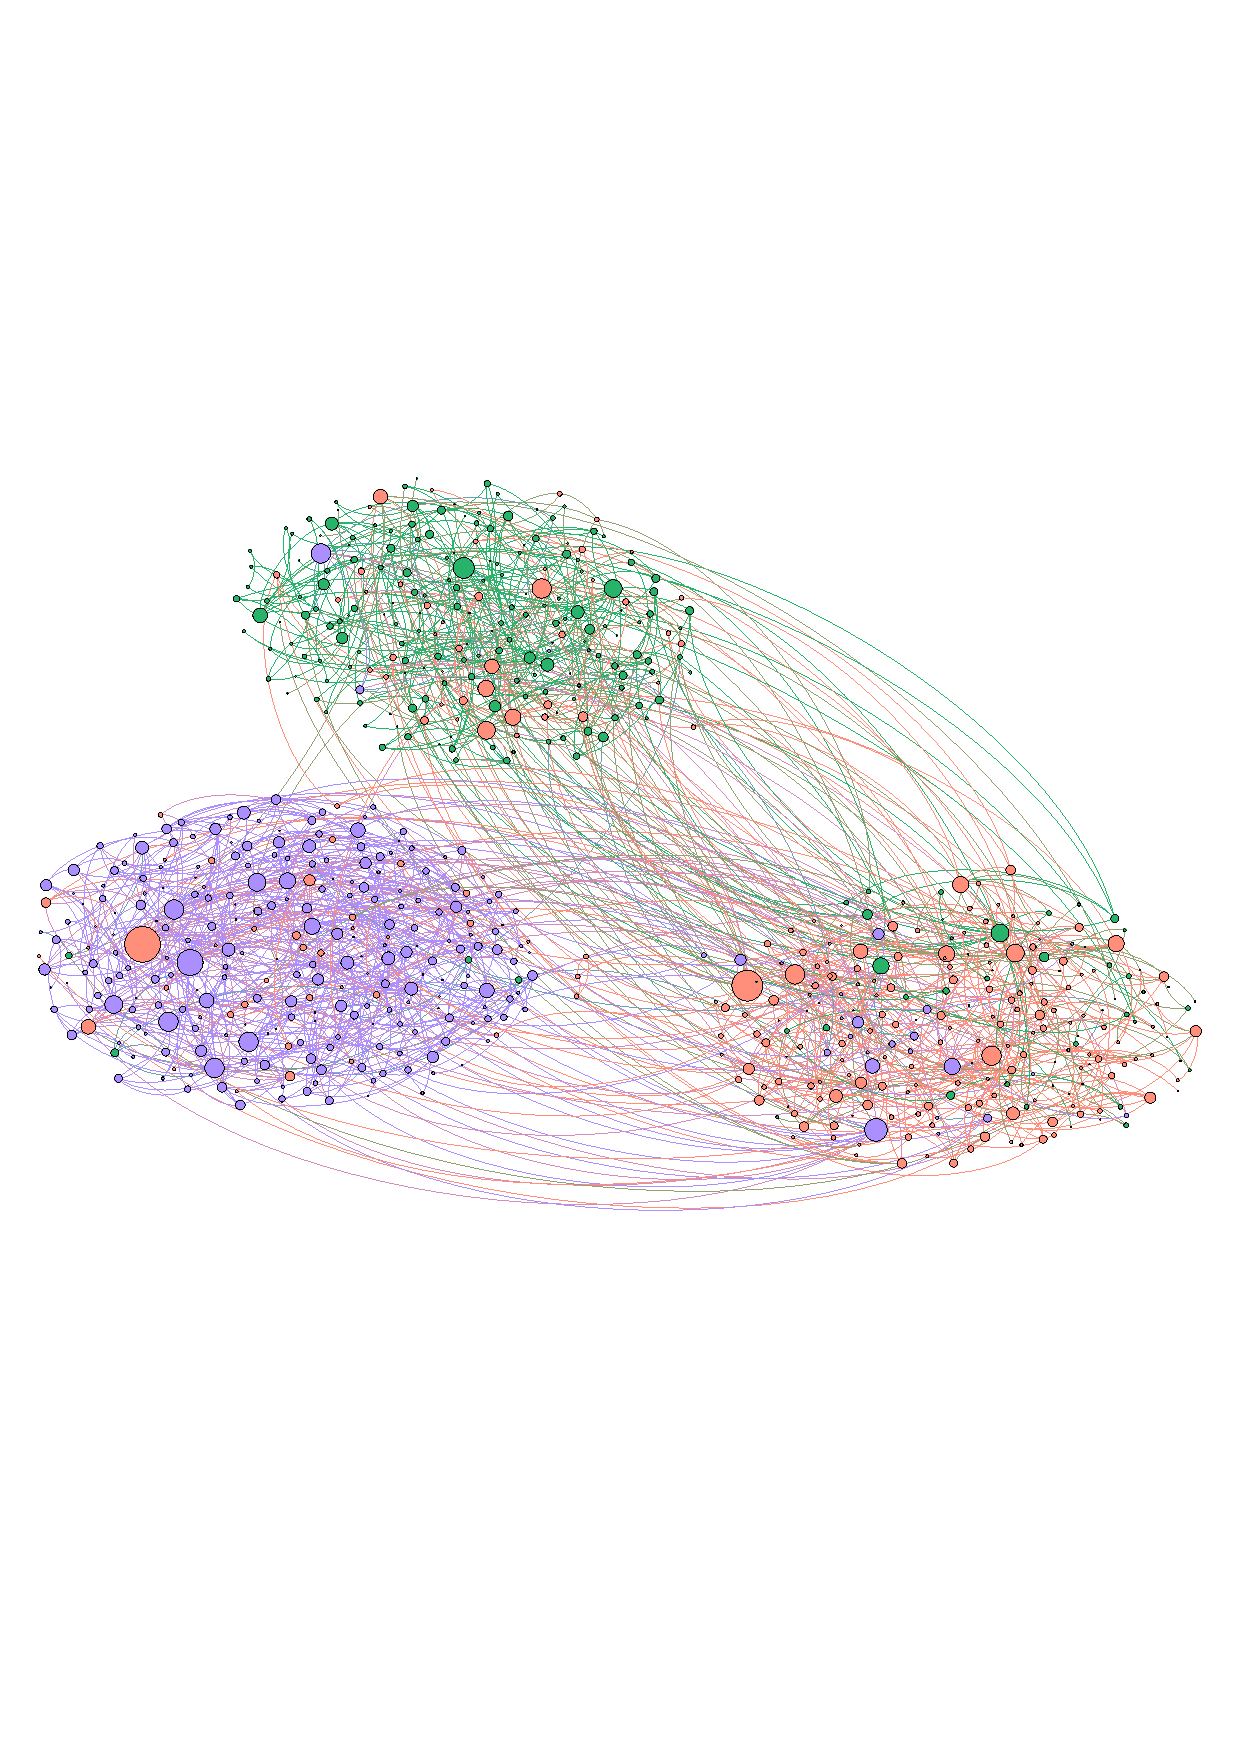
\includegraphics[width=.48\textwidth]{./figure/community2.pdf}
	\caption{论文引用数据(DBLP)的社团及社团演化示意图}
	\label{fig.3}
\end{figure}

目前动态网络社团检测的主流方法将侧重点放在了第二个问题上,根据目前主流的动态复杂网络社团检测方法的本质不同,本文将这些主流方法做出了分类,如表\ref{tab.2.1}所示,增量聚类方法根据不同相邻快照之间的节点和边的变化定义不同的目标函数,增量更新社团信息;进化聚类方法结合了当前网络快照之前的一个或几个快照的信息,来进行当前网络快照的社团检测;而生成模型方法则针对网络以及社团的生成机制进行建模并进行推断,并将动态网络的社团检测问题转化为模型的参数估计问题,从而进行社团检测。
\begin{table}[!htbp]
	\centering
	\caption{主流动态社团检测方法}
	\begin{tabular}[width=\textwidth]{lp{3cm}p{2.5cm}p{2.5cm}p{2cm}}
		\hline
		动态社团检测&核心思想&方法优势&方法不足&代表性工作\\
		\hline  %在第一行和第二行之间绘制横线
		增量聚类方法&将动态网络快照之间社团的变化转化为节点和边的变化,通过定义不同目标函数,增量更新节点的社团归属&复杂度低、对于局部结构变化较多的网络处理更加精准&过于依赖模型定义的目标函数,对网络中的噪声敏感&GraphScope~\cite{sun2007graphscope} GraphTinker~\cite{jaiyeoba2019graphtinker} TILES~\cite{rossetti2017tiles} 模块度优化~\cite{lyf2015} \\
		进化聚类方法&融合动态网络当前快照之前的一个或几个快照社团结构信息,保持社团关系变化的平滑性&融合了历史快照信息,社团检测结果较好&进行大量的网络信息重复计算,复杂度较高&Genlouvain~\cite{jutla2011generalized} PisCES~\cite{liu2018global} DYNMOGA~\cite{folino2014evolutionary} 进化谱聚类~\cite{huang2019community}\\
		生成模型方法&基于隐马尔科夫模型假设,利用生成模型对动态网络进行建模,将社团检测问题转化为参数估计问题&具有严格的理论解释和意义、模型可用于多种网络分析任务&模型优化较困难,同时概率模型的参数较多,参数域较大,因此复杂度较高&动态隐空间模型~\cite{sewell2017latent,yang2015a},动态随机块模型~\cite{yang2011detecting,pensky2017spectral,wu2019dynamic}\\
		\hline % 在表格最下方绘制横线
		
		\label{tab.2.1}
	\end{tabular}
	
\end{table}

\subsection{增量聚类方法}
增量聚类的主要思想是,首先,在动态网络的第一个快照上执行静态社团检测算法,然后根据网络在接下来的快照中的节点和边的变化调整节点的社团归属。Sun等人提出了GraphScope~\cite{sun2007graphscope}方法,GraphScope避免了额外的参数设置(如社团个数、节点的社团转移阈值等),利用信息论的最短描述长度来判别节点的社团变化,并通过处理流数据提升了算法的计算效率。GraphScope在二分网络上具有很好的效果。GraphTinker~\cite{jaiyeoba2019graphtinker}通过定义多种不同的哈希策略来提升传统增量聚类的运行效率和精度,较传统增量聚类运行效率有两倍以上的提升。TILES~\cite{rossetti2017tiles}利用标签传播来刻画节点在网络中的局部变化,以此来减少计算节点在不同时间片上的社团变化的复杂度,同时,标签传播方法还一定程度上避免了单纯的定义目标函数造成的错误累积问题,于此同时,TILES还通过定义不同的触发机制来判定社团的分裂以及合并等演化行为。而IDCD~\cite{lyf2015}方法则通过对第一个时间片的网络对边进行重要性排序,然后通过最大化模块度来检测第一个时间片的社团结构,随后根据后续时间片节点的Jaccard相似度对相应节点的边进行排序,随后按照重要性降序对边关联的节点进行社团划分,该算法的复杂度很低,但是在真实网络中效果并不好。

总的来说,增量聚类在动态网络社团检测中具有效率高,易由静态网络社团检测方法进行迁移等优点,但是其缺点也很明显,由于增量聚类依赖于定义的目标函数,因此存在错误率累积的问题,这使得该方法对数据的噪声过于敏感,因此大部分增量聚类的方法在真实数据中的效果都不是很好。

\subsection{进化聚类方法}

进化聚类方法的主要思想是,该类方法认为动态网络在相邻的时间片时不会发生突变的,因此动态网络的社团结构在相邻时间片或某足够小的时间窗口内的变动是平滑的,所以这类方法在检测某网络快照的社团时,会融合当前快照之前的社团信息,以此来保持节点社团变化的平滑性。Chakrabarti等人首次提出了进化聚类\cite{chakrabarti2006evolutionary},并定义了进化聚类的框架。其本质可表示为
\begin{equation}
	\begin{split}
		Loss = \alpha \times HL + (1-\alpha) \times PL
	\end{split}
\end{equation}
其中Loss表示进化聚类目标函数的整体损失,HC表示当前快照的社团检测结果与上一快照社团检测结果变化的损失,而PC则为当前网络快照的社团检测目标函数的损失,$\alpha$则代表平衡因子,用来控制历史快照对当前快照社团检测的影响力。

 Genlouvain~\cite{jutla2011generalized}继承自Mucha等人2010年在Science上提出的广义网络质量函数框架~\cite{mucha2010community},模型通过定义动态网络连续时间片的\textit{null model},从而得到了动态网络的模块度的定义$Q_{multislice}$。利用动态网络模块度优化,进而得到动态网络的社团划分结果。Folino等人则提出了DYNMOGA~\cite{folino2014evolutionary},DYNMOGA方法基于多目标优化将进化聚类目标函数的两个部分建模为多目标优化问题,并利用遗传算法对模型进行求解。Liu等人提出了PisCES~\cite{liu2018global}方法,通过特征向量平滑的方法约束动态网络的社团在相邻时间片变动尽可能变小,同时考虑到同社团内节点的异质性,PisCES融入了节点的度使其更能适应真实世界网络。 Huang等人~\cite{huang2019community}则结合了Fiedler特征向量与一定时间窗口的正则化拉普拉斯矩阵,进一步用谱聚类的方法进行社团检测。
 
 总的来说,通过融合了动态网络历史社团信息,进化聚类的效果要优于增量聚类方法,但是由于进行社团计算时需要引入更多信息,其复杂度要高于增量聚类。同时,由于参数$\alpha$的存在,使得模型需要进行额外的调参,不利于实际使用。
%\begin{equation}
%\begin{split}
%& Q_{multislice} = \frac{1}{2\mu}\sum_{ijsr}[(A_{ijs}-\gamma_s \frac{k_{is}k_{js}}{2m_s}\delta_{sr})+\delta_{ij}C_{jsr}]\delta(g_{is},g_{jr}) \\
%\end{split}
%\end{equation}

\subsection{生成模型方法}

生成模型方法认为节点的社团转移服从隐马尔科夫假设,通过对复杂网络进行概率建模,来构建网络的生成机制,进而将动态网络的社团检测转化为概率模型的参数估计问题。这部分的方法分类两个大类,分别为隐空间模型和动态随机块模型。

\textbf{隐空间模型}认为,节点的社团划分可以通过将节点在网络中的结构映射到多维的欧式空间中使其变得可分,进而通过利用传统机器学习聚类或者分类算法可以对其进行划分。Daniel K. Sewell等人~\cite{sewell2017latent}提出了动态网络有向和无向两个隐空间模型,定义了不同的距离函数,利用MCMC采样对模型进行求解。Yang等人\cite{yang2015a}针对非负矩阵分解以及谱聚类等利用矩阵计算的隐空间模型提出了一个新的惩罚项,用以提升这些方法通过半监督学习对不完全数据进行社团检测的效果。

而\textbf{动态随机块模型}则继承自随机块模型,有Yang等人\cite{yang2011detecting}于$2011$年通过加入社团转移矩阵A将随机块模型扩展到了动态网络。动态随机块模型认为动态网络中的任意两个节点有边的概率只与节点所在的社团有关,一个节点在一个时间片只能属于一个社团,同时在同一个社团的两个节点在社团检测与社团演化行为上是完全等价的。基于以上假设,得以构建动态随机块模型DSBM,模型通过吉布斯采样结合模拟退火算法进行参数估计,进而得到每个节点在每个时间片上的社团归属。DSBM在进行参数估计之前需要提前指定社团个数,这在真实数据进行社团检测时是不现实的,因此Tang等人~\cite{tang2014detecting}提出了DBTDP,不用社团转移矩阵决定节点的社团转移,而是通过狄利克雷过程刻画节点的转移,利用中国餐馆过程对模型进行模型选择,从而实现了模型自动确定社团个数。动态随机块模型的另一个假设,即一个节点在一个时间片只能属于一个社团,在某些真实场景中也是不合理的,比如大学里每个人可以参与多个社团,或者一个人可以有多种兴趣等等。针对这种场景,Xu\cite{xu2013dynamic}等人扩展了著名的混合随机块模型MMSB,构建了动态混合随机块模型DMMSB。而Yu\cite{yu2018detecting}等人提出了融合节点变化倾向的动态度修正随机块模型,解决了动态随机块模型第三个假设的缺陷,即同一个社团内的节点在社团转移中是完全等价的,模型融入了节点的度来修正不同节点之间连边的异质性;而对于同一社团内节点异质性的把握,Xunxun Wu等人\cite{wu2019dynamic}提出了DPSBM,给出了不同的思路,通过在动态随机块模型中引入了度衰减参数,并假设该参数随时间变化服从半正太分布而演化,从而刻画出了动态网络中节点度分布服从power law的无标度属性。

总体来说,生成模型的方法通过对网络的生成机制进行建模,从而探究了网络生成的本质,使其根据有可解释性,然而由于是对整个网络进行建模,因此其参数数量较增量聚类和进化聚类更大,其参数的解空间更大。同时由于其模型结构的复杂性,使得对模型的参数估计多为MCMC对解空间进行全局搜索,因此其效果更好的同时,复杂度也比前两种方法更高。

\section{动态网络社团演化}

针对动态网络社团检测的第三个子问题,即动态网络相邻时间快照的节点社团演化分析,也一直有人在关注,但是目前还处于起步阶段,对节点随着时间发生社团转移的本质依然没有统一的定论。Dakiche等人\cite{dakiche2019tracking}就社团演化追踪进行了总结,本小结参考他们的总结并结合实际将动态网络社团演化划分为独立社团演化、非独立社团演化以及同步社团演化进行三大类,如表~\ref{tab.2.2}所示。可以看到表中的部分方法与上一小节有重叠,因为动态网络社团检测的不同方法侧重点不同,但是对社团检测以及社团演化一定都有涉及。

\begin{table}[htbp]
	\centering
	\caption{动态社团演化方法}
	\begin{tabular}[width=\textwidth]{lp{3cm}p{2.5cm}p{2.5cm}p{2cm}}
		\hline
		动态社团演化&核心思想&方法优势&方法不足&代表性工作\\
		\hline  %在第一行和第二行之间绘制横线
		独立社团演化&即熟知的两步法,在每个时间片单独进行社团检测,随后对相邻时间片进行社团匹配&容易从发展较好的静态网络社团检测算法进行扩展,可以独立定义社团演化机制&过于依赖定义的社团演化机制,对社团检测效果没有帮助& 基于社团演化事件的方法~\cite{asur2009an,palla2007quantifying,brodka2013ged} \\
		非独立社团演化&假设社团在相邻时间片上不会发生突变,在进行社团检测时定义相应的惩罚项约束社团的演化&社团演化由惩罚函数进行控制,可以加强社团检测效果&进行大量的网络信息重复计算,复杂度较高,无法处理网络的突变&进化聚类~\cite{jutla2011generalized,liu2018global,folino2014evolutionary}  关键节点追踪~\cite{gao2016evolutionary}\\
		同步社团演化&基于隐马尔科夫模型假设,利用生成模型对动态网络进行建模,同时建模社团结构以及其演化规则&具有严格的理论解释和意义、模型可用于多种网络分析任务,社团检测结果与社团演化相互增强&模型优化较困难,同时概率模型的参数较多,参数域较大,因此复杂度较高&DSBM~\cite{yang2011detecting} 涂色优化法~\cite{tantipathananandh2011finding} DPSBM~\cite{wu2019dynamic}\\
		\hline % 在表格最下方绘制横线
		
		\label{tab.2.2}
	\end{tabular}
	
\end{table}

\subsection{独立社团演化}

独立社团演化将动态网络的社团检测与社团演化分别进行独立的计算,在每个时间片执行静态社团检测方法,随后在相邻时间片处理两个社团集合的匹配问题。社团匹配的方法大多基于相似性指标进行匹配,同时这类方法还定义了社团的演化事件,通过确定社团的演化事件来追踪社团的演化。Asur等人\cite{asur2009an}定义了社团的五个可能事件,分别为社团的消失、形成、延续、分裂和合并。而Palla等人\cite{palla2007quantifying}则提出了社团的六种演化事件,分别为增长、缩小、出生、消亡、分裂和合并。在此之后,Brodka等人\cite{brodka2013ged}则融合了前两种事件,提出了社团增长、缩小、延续、出生、消亡、分裂和合并七种演化事件。对于这些事件的检测,以上三组团队均选择在相邻两个时间片进行检测,而Tajeuna等人~\cite{tajeuna2015tracking}则选择在整个动态网络上进行社团演化事件检测。

同时对于相邻时间片的社团匹配,也有不同的社团相似性指标,如Greene等人\cite{greene2010tracking}利用了Jaccard系数计算相邻时间片社团的相似性;而Brodka等人\cite{brodka2013ged}则提出了inclusion度量来计算相邻时间片的社团匹配度;于此同时,Tajeuna等人~\cite{tajeuna2015tracking}定义了名为互转换指标的另一种相似性度量。

独立社团演化可以自由定义社团演化追踪的方法方式,对社团演化事件的追踪也更加的细致。但是社团演化行为是建立在每个事件片上社团检测足够准确的基础上的,割裂了社团演化和社团检测,这类方法的动态社团检测结果往往在真实数据集中表现不好,因为真实世界的动态网络往往具有较高的噪声,同时这类方法也考虑不到社团演化对每个时间片社团的影响。

\subsection{非独立社团演化}
非独立社团演化将社团演化融入到相邻的时间片,以此来增强社团检测效果。这部分包括上一小节介绍的进化聚类的相关方法,如Genlouvain~\cite{jutla2011generalized}PisCES~\cite{liu2018global}DYNMOGA~\cite{folino2014evolutionary}等。同时,非独立社团演化还包括了通过追踪关键节点的方法来追踪社团演化,如Gao等人~\cite{gao2016evolutionary}定义了每个社团的领导节点和跟随者节点,并假设每个社团的演化行为是由领导节点的行为导致的,这使得社团的追踪演化为了对领导节点的追踪。

这类方法在相邻社团融合了社团检测和社团演化,对社团演化的追踪也有一定独到之处,但是这种方法由于其前提假设使得其无法应对网络突变,也并不能很好的把握社团演化的本质。
\subsection{同步社团演化}

同步社团演化通过对网络的建模,同时构建了动态网络社团的产生和社团的演化。如DSBM~\cite{yang2011detecting}通过社团转移矩阵$A$来刻画动态网络中节点的社团转移,通过对$A$的估计,即可得到节点在相邻时间片的演化倾向。然而其社团转移矩阵$A$并不随时间变化,因此并不能刻画节点演化倾向的变化。DPSBM~\cite{wu2019dynamic}则利用其构建的节点度衰减参数$\delta$来修正不同时间片不同节点社团转移的异质性,从而利用$\delta$刻画整个网络节点的社团转移,进而把握住社团的演化。除了以上方法,同步社团演化也存在一些启发式优化方法,如Tantipathananandh等人~\cite{tantipathananandh2011finding}将动态网络社团检测建模为连续的图染色问题,通过求解染色问题来刻画每个时间片的社团以及社团的演化。然而该方法是NP的时间复杂度,虽然作者利用一些启发式方法对求解过程进行了优化,其复杂度依然较高。

同步社团演化结合了社团检测和社团演化,对社团检测与社团演化的效果都比较好,但是由于大部分方法建模的侧重点放在了社团检测,对于社团演化事件以及演化行为的更细节的把控程度以及社团演化的本质探究并不深入。同时概率模型的复杂性使得其求解较困难。


\section{城市风险计算}

针对城市风险的研究由来已久,早在$2007$年,吴竹就在政法学刊上发表了《群体性事件预警指标体系研究》~\cite{wu2007group},文章认为,群体性事件预警是通过对社会系统中的不良因素或者负面因子的检测和评估而形成的,因此吴竹在文章中构建了涉及城市群体性事件预警指标体系,包括了六个子系统下的$67$个具体指标,由于这些指标涉及层面太过广,计算难度很大。而随着互联网的发展,网络空间也成为了城市风险的重要因素之一。王连强~\cite{WangLianqiang2016message}在$2006$年提出了信息安全风险的评估方法框架,框架包括了信息安全风险评估方法ISRAM,定义了信息安全风险评估的计算框架以及平台实现;同时还包括了安全风险评估因素的分类研究等。然而其定义的信息安全风险评估计算涉及的变量及因素较多且框架并没有形成完整的系统,可适用性并不好。同时该框架仅仅涉及信息安全风险,并不与城市风险形成关联。龚俭等人~\cite{gongjian2017network}$2017$在软件学报发表了《网络安全态势感知综述》,该综述中提出了网络安全态势感知框架,该框架的态势察觉-态势理解-态势评估模块不仅在网络安全态势感知中获得大部分人的认同,同时给物理空间安全态势感知也提供了有效的参考。文章也同时提出了利用聚类的方法将相似性的警报进行聚类同一整合,减少系统警报数量。

而随着计算机算力的指数性提升,利用计算机结合有效的算法对城市风险进行计算是目前城市风险计算的显而易见的发展方向。然而由于城市数据的维度广,不同层面的数据之间交互复杂,单纯的机器学习算法由于其对数据单元的i.i.d假设导致其并不能准确的计算城市风险。另一方面,城市风险计算方式通过传统的群体性事件预警或者评估方法需要的资源以及计算量非常大,并不能做到有效且实时。因此通过复杂网络对城市数据进行建模,进而利用复杂网络中的相关算法对城市风险进行计算评估是合理且最行之有效的。

利用复杂网络对城市系统进行建模的研究由来已久,如利用复杂网络分析台风对城市的影响~\cite{chenchangkun2012taifeng}、利用复杂网络对电力系统进行建模并分析其脆弱性~\cite{2014electric}、利用复杂网络建模城市道路网络,并分析其脆弱性~\cite{zhangshude2014}等等。由此可见,复杂网络的脆弱性计算~\cite{gou2016topological}应用到城市系统中,可以在很大程度上发现城市的潜在风险。

\begin{figure}[htbp]
	\centering
	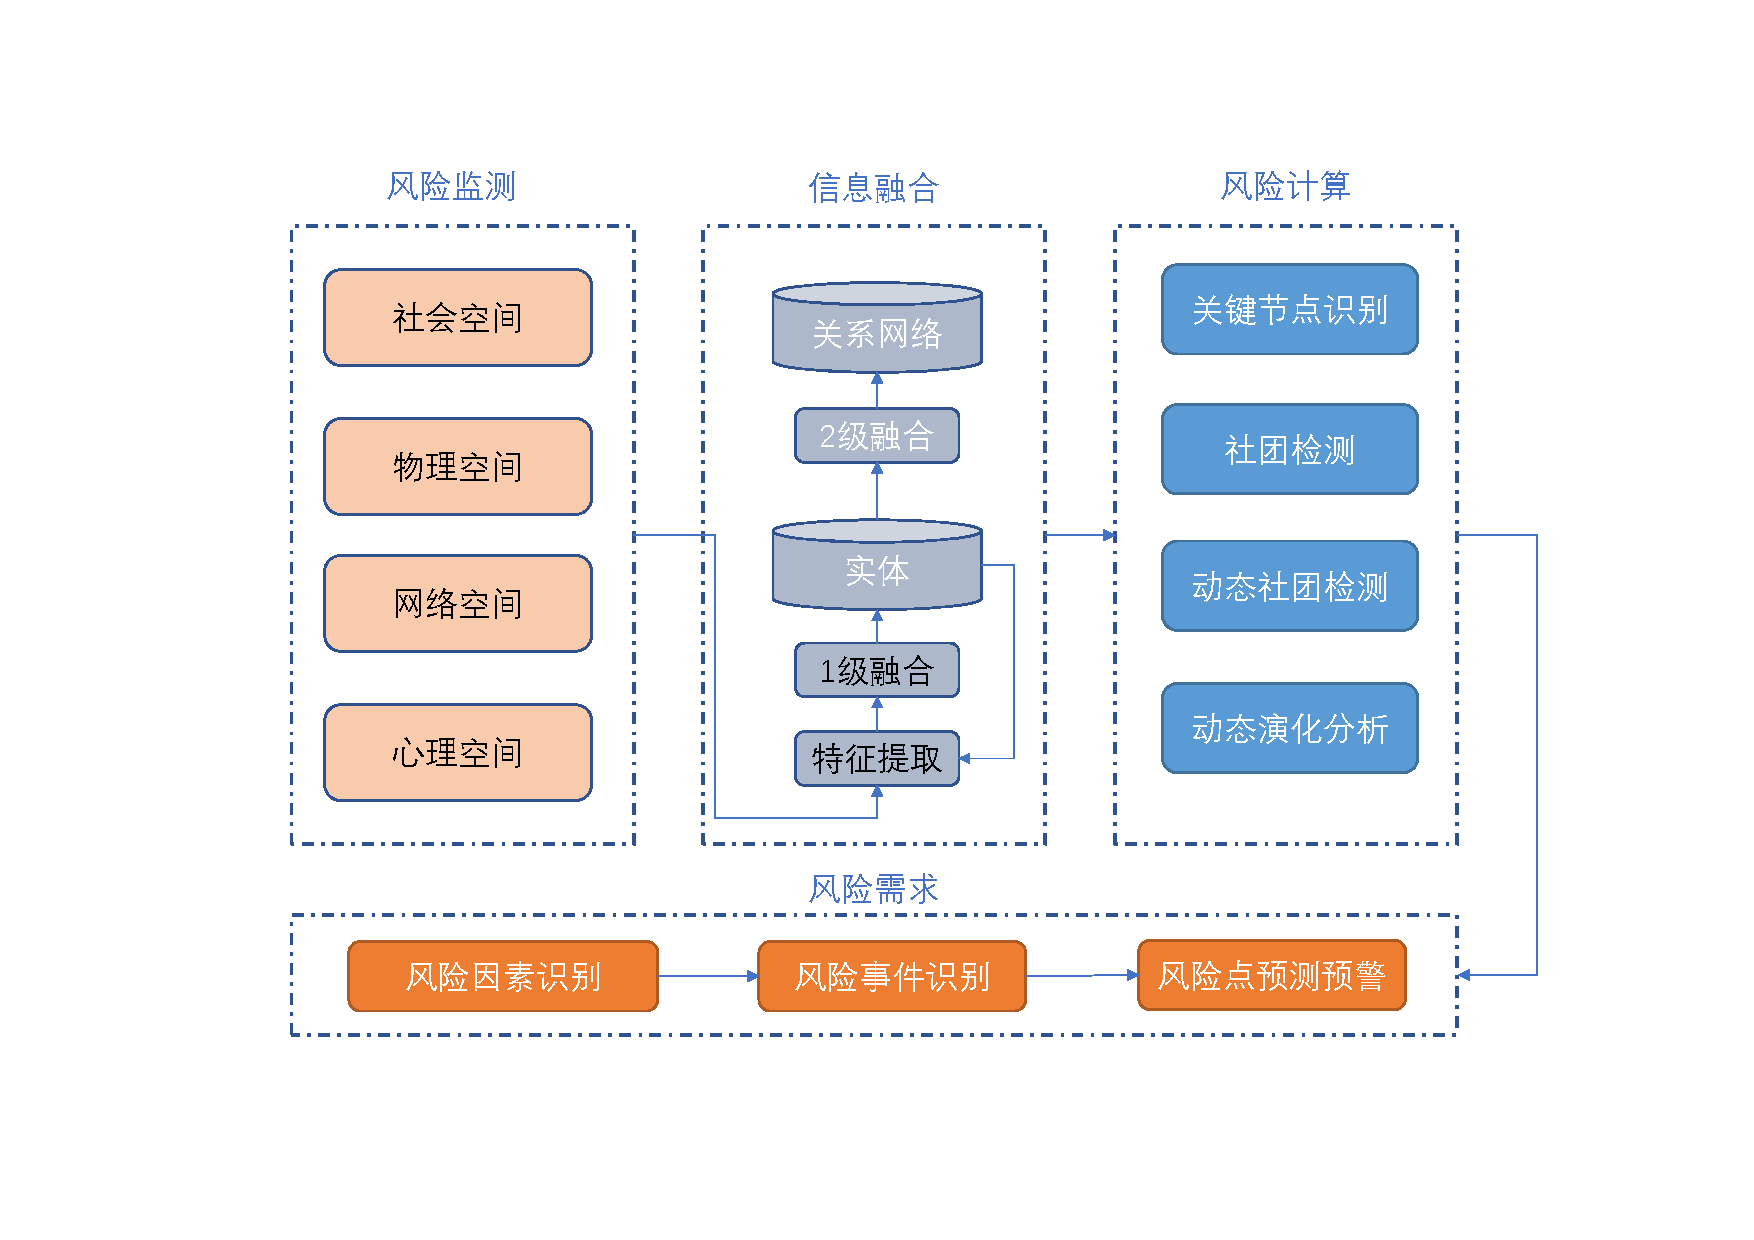
\includegraphics[width = 0.9\textwidth]{./figure/framework2.pdf}
	\caption{风险计算框架图}
	\label{fig.2}
\end{figure}

本文的风险计算研究框架如图\ref{fig.2}所示,通过整合多渠道的城市风险计算流程总结整合而成,首先监测多元空间的数据,并通过信息融合将数据进行预处理、数据对齐等步骤将潜在风险的数据融合处理为实体,进一步经过二级融合将数据构建成复杂网络。根据不同的风险需求,复杂网络算法会在其中起到各不相同的作用。

而动态网络社团检测则能够处理风险事件识别或风险因素识别的风险需求,通过对风险网络中的节点进行动态社团检测,并进一步进行事件提取,随后利用相关的打分算法对不同事件进行打分,随后筛选出潜在的风险事件~\cite{moriano2019community-based}。也可以利用社团演化分析,判断团体的发展走向,结合网络脆弱性指标或者节点重要性指标,综合分析城市中某些团体的潜在威胁。

%\section{符号表示}


\section{本章小结}
本章首先介绍了复杂网络分析的发展历程及其主要任务,随后聚焦于复杂网络分析中的社团检测的相关研究。接着针对动态网络社团检测的目前研究现状以及存在的主要问题进行了阐释说明。最后,本章介绍了风险计算的发展现状与城市风险计算和社团检测的紧密联系进行了说明。
